% example with anatomy of a decision tree
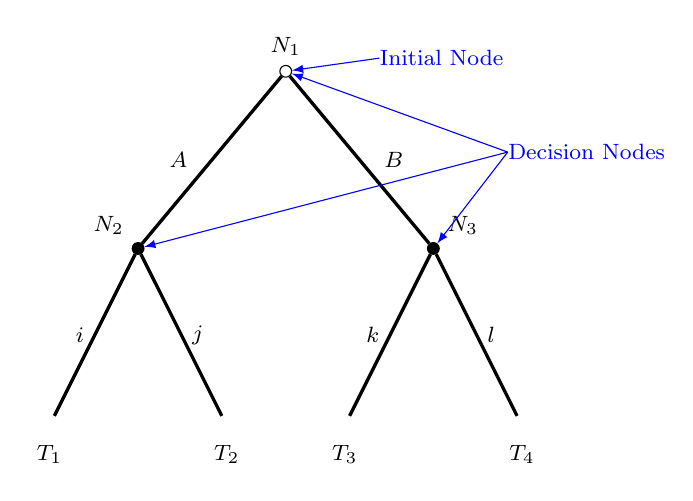
\begin{tikzpicture}[scale=1.5,font=\footnotesize, edge from parent/.style={draw, very thick}]
    \tikzstyle{solid node}=[circle,draw,inner sep=1.5,fill=black]
    \tikzstyle{hollow node}=[circle,draw,inner sep=1.5]
    \tikzstyle{level 1}=[level distance=15mm,sibling distance=2.5cm]
    \tikzstyle{level 2}=[level distance=15mm,sibling distance=1.5cm]
    \tikzstyle{level 3}=[level distance=15mm,sibling distance=1cm]
    
    \node(0)[hollow node,label=above:{$N_1$}]{}
        child{node(1)[solid node,label=above left:{$N_2$}]{}
            child{node[label=below:{$T_1$}]{} edge from parent node[left]{$i$}}
            child{node[label=below:{$T_2$}]{} edge from parent node[right]{$j$}}
            edge from parent node[left,xshift=-5]{$A$}
        }
        child{node(2)[solid node,label=above right:{$N_3$}]{}
            child{node[label=below:{$T_3$}]{} edge from parent node[left]{$k$}}
            child{node[label=below:{$T_4$}]{} edge from parent node[right]{$l$}}
            edge from parent node[right,xshift=5]{$B$}
        };

    \draw[<-,>=latex, color=blue](0)--(8:8mm)node[inner sep=0,right]{Initial Node};
    \draw[<-, >=latex, color=blue](1)--(-20:20mm)node[inner sep=0, right]{Decision Nodes};
    \draw[<-,>=latex, color=blue](2)--(-20:20mm){};
    \draw[<-,>=latex, color=blue](0)--(-20:20mm){};
\end{tikzpicture}